\title{Синтаксический анализ графов с помощью парсер-комбинаторов}
\titlerunning{Синтаксический анализ графов с помощью парсер-комбинаторов}
\author{Смолина Софья Константиновна}
\authorrunning{С.К. Смолина}
\tocauthor{С.К. Смолина}
\institute{Санкт-Петербургский государственный электротехнический университет «ЛЭТИ» им. В.И.Ульянова (Ленина)\\
\email{sofysmol@gmail.com}}
\maketitle

\begin{abstract}
Запросы к графовым базам данных могут быть сформулированы как
задача поиска путей в графе, удовлетворяющих некоторым ограничениям.
Часто такие ограничения задаются грамматиками. В таком случае задача
сводится к поиску путей в графе, которые соответствуют строкам в
некотором языке. Такую задачу назовем синтаксическим анализом графов.
Существует несколько подходов решения данной проблемы, но все они
подразумевают использование парсер-генераторов, что не всегда удобно. В
нашей работе к задаче анализа графов была адаптирована библиотека парсер-комбинаторов Meerkat.
\end{abstract}

\section*{Введение}

Синтаксический анализ, как правило, используется для построения структурного представления кода с использованием грамматики, описывающей разбираемый язык. Абстрактное синтаксическое дерево, являющееся результатом работы синтаксического анализатора, в дальнейшем используется для проведения статического анализа кода или же в каких-то других целях. Как правило, на вход синтаксическому анализатору подаётся линейная последовательность токенов, представляющая код программы. Однако могут возникать ситуации, когда вход не может быть представлен линейно. Такие ситуации могут возникать, например, при автоматической генерации кода. Генерация может происходить в циклах, с использованием условных операторов или строковых операций. Поэтому для описания генерируемых цепочек можно использовать конечный автомат, порождающий цепочки, который уже не будет являться линейным. Такую задачу будем называть синтаксическим анализом регулярных множеств.

Кроме этого, ещё одной областью, где может быть применим синтаксический анализ регулярных множеств, является бионформатика. Одной из часто возникающих задач в биоинформатике является классификация организмов, находящихся в образцах, полученных из окружающей среды~\cite{bioRNA}. По образцам строится метагеномная сборка, которая содержит в себе смесь из ДНК всех содержащихся в сборке организмов. В свою очередь ДНК является последовательностью символов в алфавите \{A, C, G, T\}. ДНК организмов, которые относятся к одному и тому же виду, содержат одинаковые подцепочки, которые и необходимо выделить, чтобы классифицировать организм. Как правило, эти подцепочки~--- это последовательности РНК. РНК может быть описана с помощью грамматики. Метагеномная сборка, в свою очередь, может быть представлена в виде графа с цепочками на рёбрах. Таким образом, в таком графе необходимо найти цепочки, выводимые в грамматике, описывающей РНК. 

Грамматики, описывающие структуру РНК, являются неоднозначными. Грамматика называется неоднозначной, если одна и та же цепочка может быть выведена несколькими способами. Такие алгоритмы синтаксического анализа как LR и LL не позволяют обрабатывать неоднозначные грамматики. Для работы с неоднозначными грамматиками существуют алгоритмы обобщённого синтаксического анализа GLR~\cite{GLR}, GLL~\cite{GLL}. В рамках проекта YaccConstructor~\cite{YaccConstructorPage, YaccConstructorPaper} был реализован алгоритм GLL, кроме того, была предложена его модификация для обработки нелинейных входных данных~--- графов. Реализованная модификация позволяет находить цепочки транспортной РНК (тРНК) в небольших метагеномных сборках, возвращая координаты начала и конца найденной цепочки. Проблема заключается в том, что грамматика для описания тРНК является сильно неоднозначной, что сказывается на производительности и точности полученных результатов. Для повышения точности можно применять конъюнктивные грамматики~\cite{ConjGrammars}, в которых для описания продукций используется операция конъюнкции. Такие грамматики расширяют класс контекстно-свободных языков и позволяют точнее описать структуру тРНК. Данная работа посвящена описанию модификаций решения на основе алгоритма GLL для работы с конъюнктивными грамматиками.

\section{Постановка задачи}
Целью данной работы является исследование применимости символьных конечных преобразователей для лексического анализа. Для ее достижения поставлены следующие задачи:

\begin{itemize}
    \item Изучить возможности библиотеки Microsoft.Automata.
\item Провести сравнение производительности алгоритма операции композиции над символьными конечными преобразователями в библиотеке Microsoft.Automata с производительностью операции композиции над конечными преобразователями в исследовательском проекте YaccConstructor.
\item На основании полученных результатов сделать выводы о применимости библиотеки Microsoft.Automata для лексического анализа в проекте YaccConstructor.
  \end{itemize}

\section{Обзор}
\lstset{basicstyle=\normalsize\ttfamily, columns=fullflexible}
В данном обзоре рассматриваются некоторые подходы к заданию принтеров и форматеров, а также плагин Grammar-Kit для IntelliJ IDEA, позволяющий по БНФ-грамматике задавать синтаксический анализатор целевого языка.
Используемые плагином грамматики рассматриваются на примере грамматики языка While \cite{paper:nielson}.

\subsection{Подходы к заданию принтеров и форматеров}
Рассмотрим некоторые подходы к заданию принтеров и форматеров.
\subsubsection{Задание форматеров по описанию синтаксиса}%Язык описания синтаксиса}
Существуют различные подходы к заданию принтеров для целевого языка.
Один из них описан в \cite{paper:tbe}.
Авторы предлагают язык описания синтаксиса, по которому можно получить и синтаксический анализатор, и принтер для языка.
Описание синтаксиса состоит из правил, которые схожи с правилами формальных грамматик, но которые также задают и стиль форматирования для данной структуры языка.
Приведенное ниже правило вывода описывает основные арифметические выражения:
{
    \lstinputlisting{codes/tbeif.txt}
    %% =================================================
    %% ПРИМЕР ПОИНТЕРЕСНЕЕ
    %% непонятно, как задаются условия форматирования
    %% =================================================
}
\noindent
Первое преобразование определяет шаблон для выражений, состоящих из чисел.
Остальные преобразования задают шаблоны для операций сложения и вычитания.
Каждое из них состоит из двух меток \lstinline{<Exp>} для подстановки выражений, арифметического знака, а также двух пробелов вокруг этого знака.
Само правило явно задает способ, которым будут отформатированы арифметические выражения полученного языка.
%При дальнейшем форматировании программ на данном языке, арифметические выражения будут иметь вид, задаваемый правилом.
Вместо пробелов можно также указать табуляции и/или переносы строк.
Недостатком данного подхода является то, что правила форматирования задаются заранее, и, чтобы их изменить, необходимо менять описание синтаксиса языка.
Кроме того, каждое такое правило задает единственный вариант форматирования данной структуры.

%\subsubsection{}
Наиболее близкий к нашей работе метод описан в \cite{paper:asf-sdf}.
Принтер языка может быть получен по ASF+SDF описанию языка \cite{paper:klint}, что представляет собой контекстно-свободную грамматику.
При этом правила форматирования не указываются.
Недостатком данного подхода является то, что при генерации принтера задается базовый стиль форматирования, и, чтобы его изменить, необходимо редактировать сгенерированный код, тогда как подход с использованием синтаксических шаблонов позволяет пользователю декларативным образом настраивать принтер.

\subsubsection{Форматеры, встроенные в IDE}
Так же широко распространены форматеры, встроенные в IDE.
Они используют множество настроек для задания стиля форматирования (рис.~\ref{ov:settings}).
Среди них: тип и размер отступов, расположение фигурных скобок в C-подобных языках, политика переноса списочных выражений на новую строку и десятки других.
Набор этих настроек выбирается разработчиком форматера на основе его представлений о возможных стилях кодирования для целевого языка.
Такие форматеры обычно тесно интегрированы с IDE, имеют высокую скорость работы, и их выразительности, как правило, достаточно для задания необходимого стиля форматирования.
Однако для поддержки нового языка необходимо определить нужный набор настроек и вручную реализовать форматер.
В случае, если пользователю необходимо придерживаться стиля кодирования некоторой существующей кодовой базы, то ему нужно самостоятельно определить значения этих настроек.
Данный недостаток отсутствует в работе \cite{paper:sformatters}, где авторы предлагают инструмент, позволяющий получить некоторые настройки форматера из существующего программного кода.
Недостатком подхода является то, что число этих настроек невелико: система позволяет определять только стиль отступов, стили именования идентификаторов, необходимое количество комментариев.
Другой подход \cite{blog:genformat} предлагает использование генетического алгоритма 
%\footnote{\texttt{https://en.wikipedia.org/wiki/Genetic\textunderscore algorithm}} 
для поиска настроек форматера в исходном коде программ на языке C.

%и в работе\footnote{\texttt{https://blog.jetbrains.com/clion/2015/11/applying-genetic-algorithms-to-automatic-code-formatting/}}. 
%Они представляют собой способы автоматического вычленения настроек форматирования из программного кода.
\begin{figure}[t]
    \centering
    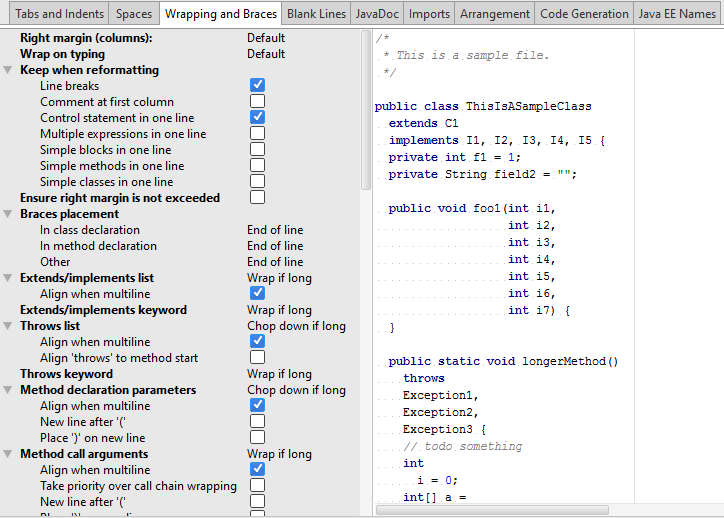
\includegraphics[width=.7\textwidth]{images/settingsjava.PNG}
    \caption{Настройки форматера языка Java в IntelliJ IDEA}
    \label{ov:settings}
\end{figure}

\subsection{Grammar-Kit}
Как уже было отмечено, для поддержки нового языка в платформе IntelliJ IDEA необходимо разработать синтаксический анализатор.
Для его генерации можно использовать плагин Grammar-Kit.
В качестве системы описания синтаксиса языка используется БНФ-грамматика.
Результатом работы плагина является код синтаксического анализатора и иерархия классов внутреннего представления. %(для IntelliJ IDEA~--- \emph{PSI-классов}).%PSI-классов.
%PSI-классом является каждая структура языка, вместе они образуют иерархию.

%Кроме того, при реализации поддержки нового языка в платформе возникает потребность в форматере.
%Мы хотим задавать принтер для языка, используя его грамматику.
% что тут еще описывать?
%\subsection{Грамматика языка While}
%Для апробации метода, описанного в \cite{paper:while}, использовался язык While, поэтому будем рассматривать грамматики, с которыми работает Grammar-Kit, на примере грамматики языка While.
Рассмотрим грамматику языка While, для которого производилась апробация метода, описанного в \cite{paper:while}.
%Рассмотрим БНФ-грамматику, использующуюся в плагине Grammar-Kit на примере грамматики языка While (рис.~\ref{ov:whileBnfFull}).
%\begin{figure}[p]
%\fvset{frame=lines,framesep=5pt}
While~--- язык программирования, содержащий следующие конструкции: чтение из стандартного потока (\lstinline{read}) и запись в стандартный поток (\lstinline{write}), оператор ветвления (\lstinline{if}), цикл с предусловием (\lstinline{while}); процедуры (\lstinline{proc}), бинарные выражения (\lstinline{binary_expr}), в том числе булевы (\lstinline{binary_bexpr}) и т. д.
% (рис.~\ref{ov:whileI},~\ref{ov:whileII},~\ref{ov:whileIII}).
\begin{figure}[h]
 %   \begin{pyglist}[numbers=left,numbersep=5pt]%, basicstyle=\ttfamily]
    \begin{lstlisting}[numbers=left, numbersep=3pt, basicstyle=\ttfamily\small, numberstyle=\tiny, frame=bottom, language={}]
whileFile  ::= proc_list stmt_list
stmt_list  ::= stmt*
proc_list  ::= procedure*
stmt       ::= skip|assign|if|while|write|read
skip       ::= 'skip' ';'
write      ::= 'write' '(' expr ')' ';'
read       ::= 'read' '(' id ')' ';'
assign     ::= id ':=' expr ';'
if         ::= 'if' '(' bexpr ')' 'then' stmt_list ('else' stmt_list)? 'fi'
while      ::= 'while' '(' bexpr ')' 'do' stmt_list 'od'
procedure  ::= 'proc' id '(' param_list ')' stmt_list 'endp'
param_list ::= ref_expr? (',' ref_expr)*
...
 \end{lstlisting}
    \caption{Грамматики языка While. Операторы языка}
    \label{ov:whileI}
\end{figure}
\noindent
На рис.~\ref{ov:whileI} представлена часть грамматики языка While, задающая множество операторов.
Рассмотрим правило грамматики, задающее оператор ветвления.
Правая часть правила состоит из терминалов \lstinline{'if'}, \lstinline{'then'} \lstinline{'('} и др.; нетерминалов: \lstinline{bexpr}, \lstinline{stmt_list}, а также условного вхождения \lstinline{('else' stmt_list)?} (то есть конструкция может отсутствовать в программах на данном языке).
Некоторые правила грамматики имеют модификаторы, которые используются для дополнительных указаний генератору синтаксического анализатора (рис.~\ref{ov:whileII}).
\begin{figure}[h]
    %\begin{pyglist}[numbers=left,numbersep=5pt]
    \begin{lstlisting}[numbers=left, numbersep=3pt, basicstyle=\ttfamily\small, numberstyle=\tiny, frame=bottom, language={}]
...
fake ar_op        ::= plus_op|mul_op
fake binary_expr  ::= expr ar_op expr 

expr              ::= factor plus_expr *
left plus_expr    ::= plus_op factor
plus_op           ::= '+'|'-'
private factor    ::= primary mul_expr *
left mul_expr     ::= mul_op primary
mul_op            ::= '*'|'/'|'%'
private primary   ::= literal_expr | ref_expr | paren_expr
paren_expr        ::= '(' expr ')'
ref_expr          ::= id
literal_expr      ::= number

fake bl_op        ::= or|and
fake binary_bexpr ::= bexpr bl_op bexpr
...
    \end{lstlisting}
    %\end{pyglist}
    \caption{Грамматика языка While. Выражения с модификаторами}%?
    \label{ov:whileII}
\end{figure}
\noindent
Модификатор \lstinline{fake} указывает системе, что не нужно генерировать код синтаксического анализатора для обработки данной структуры, однако генерируется иерархия классов внутреннего представления, \lstinline{private} указывает, что не будет сгенерирована иерархия классов, \lstinline{left} используется для поддержки левоассоциативности, а также некоторые другие\footnote{Посмотреть полный список можно по адресу \texttt{https://github.com/JetBrains/Grammar-Kit}}.
Модификатор \lstinline{private} используется для правил грамматики, которые не имеют представления в синтаксическом дереве.
Среди них те, которые используются для устранения левой рекурсии.
%которые не влияют на синтаксис языка, например, такие, которые используются для устранения левой рекурсии.
Например, на рис.~\ref{ov:whileExpr} представлено описание правил с рис.~\ref{ov:whileII} (строки 5--14), но в более естественной для человеческого восприятия леворекурсивной форме.
\begin{figure}[h]
    %\lstinputlisting{codes/whileExpr.txt}
    %\begin{pyglist}[numbers=left,numbersep=5pt]
    \begin{lstlisting}[numbers=left, numbersep=3pt, basicstyle=\ttfamily\small, numberstyle=\tiny, frame=bottom, language={}]
expr         ::= plus_expr | mul_expr | paren_expr | ref_expr | literal_expr
plus_expr    ::= expr plus_op expr
plus_op      ::= '+'|'-'
mul_expr     ::= expr mul_op expr
mul_op       ::= '*'|'/'|'%'
paren_expr   ::= '(' expr ')'
ref_expr     ::= id
literal_expr ::= number
    \end{lstlisting}
    %\end{pyglist}
    \caption{Грамматики языка While. Выражения в естественной леворекурсивной форме}
    \label{ov:whileExpr}
\end{figure}
\noindent
Однако грамматика, с которой работает Grammar-Kit, не должна содержать леворекурсивных правил.
Устраняя левую рекурсию, мы получим описание выражений на рис.~\ref{ov:whileII} (строки 5--14).
Кроме того, появляются новые правила, которые с точки зрения синтаксического анализа (а следовательно, и форматирования) являются избыточными.
В данном случае такими являются \lstinline{factor} и \lstinline{primary} на рис.~\ref{ov:whileII}.
\begin{figure}[b]
    %\begin{pyglist}
    \begin{lstlisting}[numbers=left, numbersep=3pt, basicstyle=\ttfamily\small, numberstyle=\tiny, frame=bottom, language={}]
{   parserClass="com.intellij.whileLang.parser.WhileParser"
    psiClassPrefix="Psi"
    psiImplClassSuffix="Impl"
    psiPackage="com.intellij.whileLang.psi.impl"
    tokens=[...]
    ...
}
...
    \end{lstlisting}
    %\end{pyglist}
    \caption{Заголовок файла с грамматикой}
    \label{ov:whileIII}
\end{figure}
% про left
Каждый файл с грамматикой языка содержит в себе заголовок, в котором описывается различная дополнительная информация: используемые в сгенерированных файлах классы, префиксы и суффиксы сгенерированных классов внутреннего представления, Java-пакеты, множество терминальных символов грамматики (\emph{tokens}) и др. (см рис.~\ref{ov:whileIII}).





\section{Разработка библиотеки для синтаксического анализа графов}
\subsection{Библиотека Meerkat}
Meerkat --- это библиотека парсер-комбинаторов, разработанная на языке программирования Scala Али Афрузе и Анастасией Измайловой~\cite{IzmCombinator} для синтаксического анализа строк. Анализ осуществляется за $O(n^3)$, где $n$ --- длина последовательности, а также осуществляется построение компактного представления леса разбора Binarized Shared Packed Parse Forest (BSPPF). В ней решены проблемы левой рекурсии, а также экспоненциальной сложности за счет использования техники мемоизации и Continuation-Passing Style, предложенной Марком Джонсоном~\cite{MemoizationInTopDown}.

\subsection{Распознаватель в стиле парсер-комбинаторов}
В терминах данной библиотеки базовый распознователь --- это функция типа $Recognizer$, которая определяется как функция $Int => Result[Int]$ (принимает значение типа $Int$ и возвращает значение типа $Result[Int]$). Базовый распознаватель --- это частичная функция, принимающее как аргумент позицию во входном потоке и возвращающее значение $success$, соответствующее успешному разбору и содержащее следующую позицию, или значение $failure$, соответствующее ошибке при анализе.

Для составления любой КС-грамматики необходимо реализовать набор базовых комбинаторов: анализаторы терминала и пустой строки, комбинаторы последовательности и правила. В библиотеке Meerkat для этих целей реализованы анализаторы $terminal$, и $epsilon$, а так же комбинаторы $seq$ и $rule$ (см. листининг~\ref{parserAll}).

\begin{listing}
\caption{Распознаватели в стиле парсер-комбинаторов}
\label{parserAll}
\centering
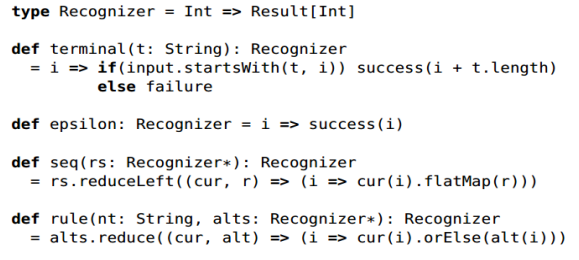
\includegraphics[width=0.9\textwidth]{Smolina/pics/combinators.png}
\end{listing}

Комбинатор $terminal$ возвращает распознаватель, который принимает индекс текущей строки и возвращает $success$ в случае, когда суффикс строки с текущего символа равен значению аргумента. Входной поток в данном случае предполагается глобальной переменной, но в реализации передаётся как параметр функции. 

Комбинатор $seq$ представляет собой последовательную композицию распознавателей. Он получает на вход текущую позицию и список распознавателей, затем применяет последовательно каждый из распознавателей к входному потоку, начиная с текущей позиции, и передает предыдущие результаты следующим распознавателям. Если какой-либо из распознавателей вернёт $failure$, то дальнейший разбор производиться не будет и комбинатор $seq$ вернёт $failure$. 

 Комбинатор $rule$ используется, чтобы определить нетерминал с именем $nt$ и списком распознавателей $alts$, которые представляют из себя альтернативы правила грамматики. Данный комбинатор принимает как параметр текущую позицию во входном потоке и применяет каждый анализатор к этому символу, пока хотя бы один не вернёт $success$. 

Для того чтобы в строго типизированных языках можно было реализовать рекурсивные распознаватели, введен дополнительный комбинатор $fix$ (см. листинг~\ref{fix}) --- комбинатор неподвижной точки.

\begin{listing}
\caption{Комбинатор fix}
\label{fix}
\centering
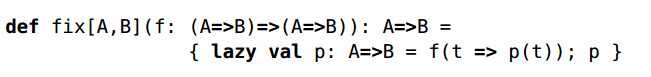
\includegraphics[width=0.9\textwidth]{Smolina/pics/fix.png}
\end{listing} 

Комбинирование элементарных анализаторов и представленных выше парсер-комбинаторов позволяет анализировать произвольную КС-грамматику и избежать зацикливания обработке леворекурсивных правил~\cite{GLL}.

\subsection{Полный перебор с использованием Continuation-Passing Style}
У базовых распознавателей есть недостатки: более высокий приоритет у первого распознавателя альтернативы и детерминизм. Из-за более высокого приоритета первого распознавателя анализ строки ``ab'' относительно грамматики $S \rightarrow A \ \$; A \rightarrow a \mid a \ b$ завершится ошибкой --- $failure$: первая альтернатива нетерминала $A$ распознает односимвольный префикс строки, после чего произойдет ошибка при проверки на конец строки, и второй распознаватель не будет применен к началу строки. Детерминизм означает, что результатом успешного распознавания всегда является единственное решение, в то время как их может быть и несколько. Порождение все возможных выводов строки возможно при помощи техники Continuation-Passing Style (CPS).

При программирования в стиле Continuation-Passing передача управления происходит через механизм продолжений. Продолжение в данном контексте представляет собой функцию высшего порядка, содержащую информацию о состоянии программы в конкретный момент времени, которое возможно сохранить и вызвать позже для перехода в данное состояние.

Для преобразования базовые распознаватели в CPS авторы библиотеки Meerkat изменили тип $Result[T]$ и сопровождающие его функции $success$ и $failure$. Любой результат теперь должно быть возможным представить как композицию двух функций, используя метод $flatMap$, или как комбинацию двух возможных альтернатив, используя метод $orElse$. Реализация в библиотеке Meerkat представлена в листинге~\ref{result}.

\begin{listing}
\caption{Result[T] для CPS распознавателей}
\label{result}
\centering
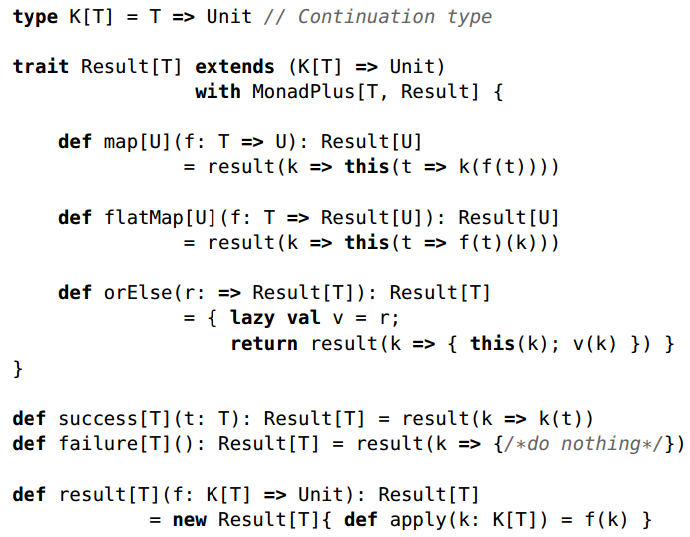
\includegraphics[width=0.8\textwidth]{Smolina/pics/result.png}
\end{listing}

CPS распознаватель принимает на вход позицию и возвращает функцию типа $Result[T]$. Данная функция принимает на вход продолжение типа $K[Int]$ и возвращает $Unit$. Продолжение в данном случае является функцией-остатком процесса распознавания. Вместо возвращения значения, распознаватель возвращает либо $success$, вызывая продолжение со следующей позиции, либо $failure$, не вызывая продолжения. Такая реализация осуществляет перебор всех возможных решений. 

\subsection{Мемоизация и поддержка левой рекурсии}
Наивный перебор всех возможных решений приводит к экспоненциальной сложности алгоритма. Библиотека Meerkat использует мемоизацию для обеспечения полиномиальной сложности, а также для решения проблемы с леворекурсивными нетерминалами.

 Мемоизацией называют механизм, который позволяет сохранять вычисленные результаты и в дальнейшем переиспользовать их. При применении распознавателя, алгоритм в первую очередь проверяет в таблице мемоизации, не было ли вычислено значение данного распознавателя в данной позиции ранее. Если вычисление происходит в первый раз, результат записывается в таблицу мемоизации. Иначе распознаватель не выполняется, а результат его работы берется из таблицы. В листинге~\ref{memo} представлен такой механизм для техники CPS, реализованный в библиотеке Meerkat.

 Функция $memo$ превращает произвольный распознаватель CPS в мемоизированный CPS-распознаватель. Мемоизированный CPS-распознаватель при каждом вызове в позиции i обращается к таблице $table$. Таблица $table$ содержит функцию для работы с продолжениями для каждого символа. В случае, когда для позиции i применяется немемоизированый распознаватель в первый раз, его модификация сохраняется и представляет собой переменную res. Результат распознавателя вычисляется только после обновления таблицы $table$. Если распознаватель был вызван в данной позиции раньше, его результат возвращается из $table$. Таким образом решается проблема экспоненциального взрыва.

\begin{listing}
\caption{Мемоизация для CPS}
\label{memo}
\centering
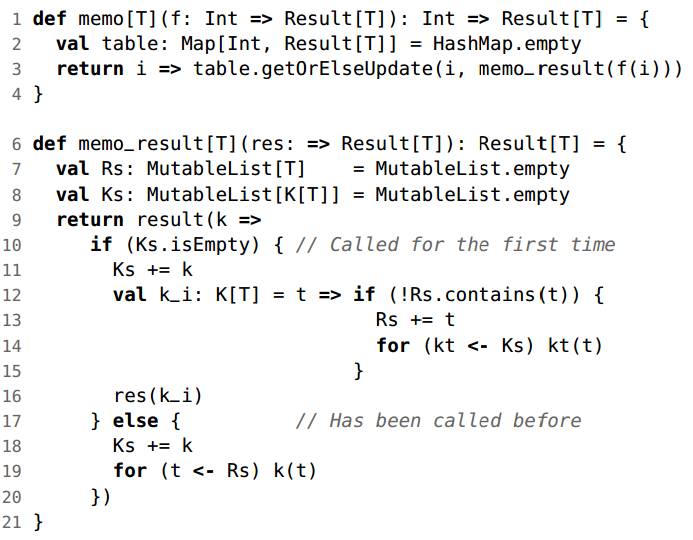
\includegraphics[width=0.8\textwidth]{Smolina/pics/memo.png}
\end{listing}

%%%%%%%%%%%%%%%%%%%%%%%%%%%%%%%%%%%%%%%%%%%%%%%%%%%%%%%%%%%%%%%%

Каждый CPS-распознаватель оперирует двумя списками: $Rs$ и $Ks$. Список $Rs$ содержит все позиции входа, созданные немемоизированным распознавателем, когда он достигает успеха, будучи примененным к позиции $i$. Список $Ks$ содержит все продолжения, которые передаются в функцию $memo\_result$, когда они вызываются в позиции $i$. Если мемоизированный распознаватель вызывается в первый раз, текущее продолжение добавляется к $Ks$, а исходный немемоизованный распознаватель вызывается с новым продолжением $k\_i$. Продолжение $k\_i$ создается только после первого вызова мемоизированного распознавателя в $i$. Каждый раз, когда немемоизированный распознаватель завершается с успехом в позиции $i$, $k\_i$ проверяет, была ли эта входная позиция получена как результат раньше, если нет, сначала записывает ее в $Rs$, а затем запускает все записанные продолжения. С другой стороны, если вызванный мемоизированный результат был вызван ранее, текущее продолжение $k$ добавляется к $Ks$ и вызывается для каждой входной позиции,записанной в $Rs$.

Теперь, когда мемоизированный леворекурсивный CPS-распознаватель вызывается во входной позиции $i$, его завершение гарантируется, поскольку соответствующий немемоизированный распознаватель никогда не будет вызван в $i$ более одного раза. В то же время, часть пути выполнения, которая привела к леворекурсивному вызову и может создавать новые позиции для левого рекурсивного распознавателя в $i$, эффективно записывается как продолжение. Каждое продолжение фиксирует следующий шаг в альтернативе после завершения текущего вызова. Продолжения будут выполняться для любой входной позиции, создаваемой леворекурсивным распознавателем в позиции $i$, до тех пор, пока создаются новые позиции ввода~\cite{IzmCombinator}. Таким образом решается проблема левой рекурсии.

\subsection{ Библиотека для синтаксического анализа графов}
Основной задачей работы является разработка решения для синтаксического анализа графа, которое позволяет не только писать запросы непосредственно в коде программы, но и получать результат этих запросов в компактной форме SPPF.

Данная работа требует решения промежуточных шагов.
\begin{enumerate}
\item Входным типом данных библиотеки Meerkat являются строки, необходимо изменить его на граф.
\item Строки можно рассматривать как линейную последовательность ребер и вершин, поэтому далее необходимо преобразовать библиотеку для анализа последовательности вершин с несколькими исходящими ребрами (деревья) с различными метками, а также графа с циклами.
\item Необходимо преобразовать библиотеку для анализа графов с одинаковыми ребрами, исходящими из одной вершины.
\item Необходимо добавить функциональность для решения частных задач синтаксического анализа.
\item Необходимо добавить функциональность для работы с графовой базой данных Neo4j.
\end{enumerate}

\subsubsection{Изменение входного типа данных на граф}


Входной последовательностью в библиотеке Meerkat являются строки. Для работы с ними разработчиками библиотеки был разработан класс $Input$, который в конструкторе получает строку. Для добавления нового типа входных данных класс $Input$ был преобразован в интерфейс $Input$, который имеет следующие методы:
\begin{itemize}
\item $startWith$: принимает на вход строку $prefix$ и позицию в последовательности $n$. Проверяет, является ли prefix префиксом суффикса строки, начинающиегося с позиции $n$;
\item $matchRegex$: принимает на вход регулярное выражение и позицию в последовательности. Проверяет, содержится ли в суффиксе строки с позиции $n$ строка, удовлетворяющая данному регулярному выражению.
\end{itemize}

Класс $InputString$ реализует интерфейс для строки, класс $InputGraph$ --- для графа. Для графа был разработан интерфейс $IGraph$, задающий методы необходимые для реализации класса $InputGraph$. Для тестирования данный интерфейс был реализован для типа данных $scalax.collection.Graph$~\cite{Graph}. Это простая в использовании реализация графа, в которой кратко и наглядно можно представить узлы и связи между ними.

\subsubsection{Преобразование системы для анализа дерева и графа с циклами}


Дерево представляет собой связный граф, в котором нет циклов. Пример дерева представлен на рис.~\ref{Graph1}. На данном этапе метки на ребрах, исходящих из одной вершины, должны быть различны. Необходимо преобразовать библиотеку для осуществления синтаксического анализа деревьев.

\begin{figure}

 \centering
 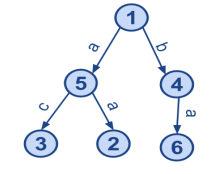
\includegraphics[width=0.4\textwidth]{Smolina/pics/Graph1.png}
 \caption{Дерево $A_1$}
 \label{Graph1}
\end{figure}

Для решения данной задачи необходимо преобразовать синтаксический анализатор терминала (см. листинг~\ref{parser1}). Данный метод принимает на вход строку-шаблон (длины $k$) и позицию во входной последовательности ($n$). Если существует подстрока, начинающаяся с позиции $k$ и совпадающая с шаблоном, то возвращается значение $success$, содержащее позицию, с которой следует продолжить разбор --- $k+n$. При обработке узла дерева просматриваются все исходящие ребра и проверяется соответствие их меток со значением терминала. Если существует ребро с соответствующим терминалом, необходимо вернуть вершину, в которую направлено ребро. Так как не для всех исходящих ребер анализ успешен, а для ситуаций успешного анализа надо возвращать позицию, то тип данных метода $startWith$ необходимо изменить с $Boolean$ на $Option[Int]$.

В графах с циклами, в отличие от деревьев, в одну и ту же вершину может существовать несколько путей, которые могут иметь циклическую структуру. В наивной реализации парсер-комбинаторов каждый путь приходилось бы пересчитывать заново, а в случае с циклом вычисление бы никогда не завершилось. Однако применение техники мемоизации совместно с CPS гарантирует вычисление каждого анализатора в каждой вершине не более одного раза. Для каждой вершины существует свой набор продолжений, который комбинируется и переиспользуется. Благодаря этим свойствам дальнейших изменений для поддержания графов с циклами не потребовалось. Циклы в графе обрабатываются подобно леворекурсивной грамматике.

Таким образом решена задача синтаксического анализа для деревьев и графов с циклами. Проиллюстрируем полученные результаты на примере 1.

\textsc{Пример 1.} 
Входной граф представлен на рис.~\ref{Graph2}, данный граф цикличен. Стартовой вершиной считаем вершину 0. Результат синтаксического анализа в соответствии с грамматикой $G_4$ представлен на рисунке~\ref{grmG4}.

\begin{figure}
 \centering
 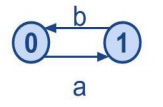
\includegraphics[width=0.2\textwidth]{Smolina/pics/Graph2.png}
 \caption{Цикличный граф $A_2$}
 \label{Graph2}у4е53 
\end{figure}

\begin{listing}
\caption{Грамматика $G_4$}
\label{grmG4}
\centering
$\begin{array}{rl}
E \rightarrow a \ b \ E \ | \ a \ b
\end{array}$
 \end{listing}

\begin{figure}
 \centering
 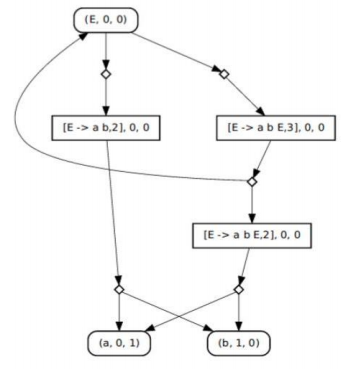
\includegraphics[width=0.4\textwidth]{Smolina/pics/Tree1.png}
 \caption{Результат применения анализатора $E$ к графу $A_2$}
 \label{Tree1}
\end{figure}

Результатом синтаксического анализа преобразованной библиотекой Meerkat является синтаксический лес разбора, представленый на рисунке~\ref{Tree1}. Из корневой вершины исходит две ветви, два возможных решения. Первое решение строка ``ab''. Второе решение соответствует рекурсивному правилу грамматики с префиксом ``ab'' с левой ветвью указывающей на корень дерева, представляя собой бесконечное множество возможных деревьев разбора.

\subsubsection{Преобразование системы для анализа графов с одинаковыми ребрами из одной вершины}


Ранее требовалась уникальность исходящих ребер из одной вершины. В этом случае из каждой вершины может существовать единственный путь, начинающийся с данного терминала. Если отказаться от данного ограничения, то таких путей может существовать несколько или не существовать вовсе, поэтому необходимо изменить тип и реализацию метода $startWith$. Теперь результатом его работы будет тип $Set[Int]$. Когда множество оказывается не пусто, будем считать, что разбор прошел успешно ($success$) иначе --- завершился ошибкой ($failure$).

Метод $terminal$ также требует изменений. Все успешные пути, полученные методом $startWith$, комбинируются при помощи $orElse$ класса
$Result$. В результате чего получаем единственное продолжение, которое возвращается для дальнейшей обработки. Пример 2 демонстрирует работу новой реализации.

\textsc{Пример 2.} 
Входной граф $A_3$ представлен на рисунке~\ref{Graph3}. Из стартовой вершины 0 исходят 3 ребра с одинаковыми метками. Проведем синтаксический анализ в соответствии с грамматикой $G_5$ в листинге~\ref{grmG5}.

\begin{figure}
 \centering
 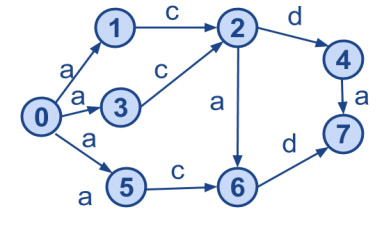
\includegraphics[width=0.6\textwidth]{Smolina/pics/Graph3.png}
 \caption{Граф $A_3$}
 \label{Graph3}
\end{figure}

\begin{listing}
\caption{Грамматика $G_5$}
\label{grmG5}
\centering
$\begin{array}{rl}
E \rightarrow a \ c \ d \ E \ | \ a \ d
\end{array}$
 \end{listing}

\begin{figure}
 \centering
 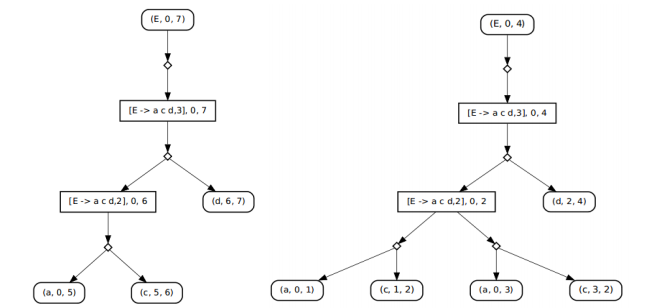
\includegraphics[width=\textwidth]{Smolina/pics/Trees2.png}
 \caption{Результат применения анализатора $E$ к графу $A_3$}
 \label{Trees2}
\end{figure}

Результат работы представлен на рис.~\ref{Trees2}. В графе $A_3$ из вершины 0 существуют 3 пути, соответствующие грамматике $G_5$ (0-5-6-7, 0-1-2-4 и 0-3-2-4). В результате получен граф SPPF, где несколько вершин выделены как начальные. Вершины, соответствующие общим подпутям при этом переиспользуются.

SPPF представляет собой компактное представление множества деревьев разбора одной строки. В случае синтаксического анализа графов необходимо построить множество деревьев разбора множества строк, что возможно сделать, если модифицировать SPPF таким образом, чтобы у него было несколько ``корневых'' узлов. За счет такого определения можно обеспечить переиспользование деревьев разбора для общих подпутей.

В библиотеке Meerkat во время анализа строится структура данных $SPPFLookup$. Она представляет собой множество уникальных узлов, создаваемых во время анализа, которые ссылаются друг на друга. При успешном результате один или несколько узлов, как в нашем случае, берутся как корни дерева.

\subsubsection{Функциональность для решения частных задач синтаксического анализа}

Раннее мы обсуждали поиск всех путей в графе, удовлетворяющих заданным ограничениям. Существуют и другие семантики запросов, при которых необходимо идентифицировать некое подмножество всех путей, удовлетворяющих ограничениям. Такими семантиками являются~\cite{Hellings}:

\begin{itemize}
\item поиск всех путей в графе;
\item поиск путей, начинающихся с какой-либо вершины из данного
множества;
\item поиск путей, завершающихся в какой-нибудь вершине из данного
множества;
\item поиск путей, начинающихся в какой-нибудь вершине множества
начальных вершин и заканчивающихся в вершине из множества
конечных вершин.
\end{itemize}

Для нахождения решений, удовлетворяющих каждой из данных семантик, не требуется изменений в процессе разбора. После построения $SPPFLookup$ необходимо произвести фильтрацию стартовых нетерминальных символов в соответствии с семантикой запроса, то есть выбрать корневые вершины, которые удовлетворяют требованиям. В итоге все вычисления производятся один раз и уже из полученных результатов выбираются необходимые. 

\subsubsection{Интеграция библиотеки с графовой базой данных Neo4j}

Было решено применить результат работы библиотеки для синтаксического анализа графов к существующей графовой базе
данных. Нами была выбрана графовая база данных Neo4j~\cite{Neo4j}. Она обладает наглядным и удобным в использовании интерфейсом, имеет REST API для доступа из любого языка программирования и большое количество пользователей по всему миру.

Для интегрирования реализован класс $Neo4jGraph$, реализующий методы интерфейса $IGraph$. Класс использует REST API для работы с базой данных, предоставленное компанией Neo4j. В качестве индексов во входном потоке используется уникальный идентификатор вершин графа.

\textsc{Пример 2.} 
Для тестирования была взята графовая база данных Wine. Фрагмент представлен на рис.~\ref{GraphWine}. Каждая вершина представляет собой вид вина, регион или тело вина. Между ними представлены два вида связи: 
\begin{itemize}
\item $locatedIn$ указывает на расположение объекта, из которого исходит ребро;
\item $hasBody$ указывает на цвет вина
\end{itemize}

\begin{figure}
 \centering
 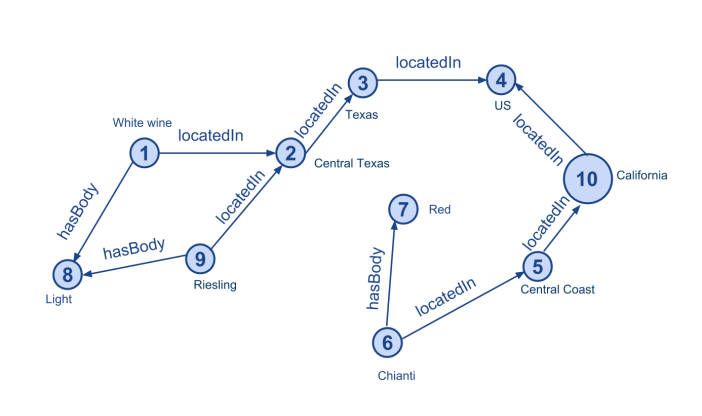
\includegraphics[width=0.9\textwidth]{Smolina/pics/GraphWine.png}
 \caption{Фрагмент графовой базы данных Wine}
 \label{GraphWine}
\end{figure}

Для того, чтобы узнать в каких регионах производят Riesling, необходимо выполнить запрос представленный в листинге~\ref{grmG6}. 

\begin{listing}
\caption{Грамматика $G_6$}
\label{grmG6}
\centering
$\begin{array}{rl}
S \rightarrow locatedId \ S | \ locatedIn
\end{array}$
 \end{listing}

В процессе работы было получено 3 пути, начинающиеся с вершины $9$ и заканчивающиеся в вершинах $2, 3, 4$. Соответствующие этим вершинам названия, соответствуют расположению регионов, где производится вино Riesling: Central Texas, Texas, US.
 
 \textsc{Пример 3.}

Другой пример, демонстрирующий необходимость в запросах, представленных в КС-грамматиках --- это поиск потомков одного поколения.

База данных моделирует семейное древо (см. рис.~\ref{GraphFamily}). Требуется найти всех потомков одного поколения: например, всех братьев и сестер конкретного узла. Нахождение всех этих потомков может быть произведено запросом в виде грамматики $G_7$ (см. листинг~\ref{grmG7}). Данная грамматика представляет собой язык правильных скобочных последовательностей, где одна скобка --- отношение ``ребенок'', другой --- отношение ``родитель''. Технически, данные в базе данных представлены таким образом, что существуют только переходы от предков к потомкам, поэтому отношение ``ребенок'' необходимо симулировать как обратное ребро. Для обработки данной ситуации был добавлен комбинатор ``not'', который осуществляет анализ в обратном направлении: от узла, в которое входит ребро, в узел, из которого исходит ребро.

\begin{figure}
 \centering
 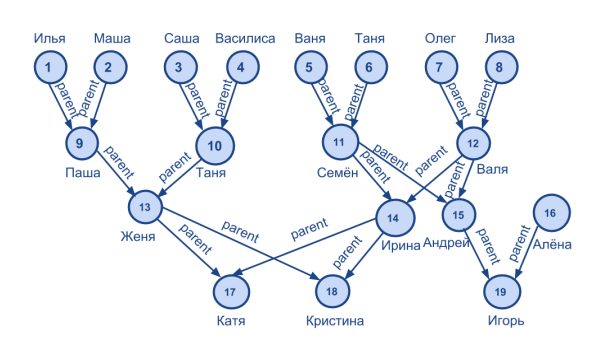
\includegraphics[width=0.8\textwidth]{Smolina/pics/GraphFamily.png}
 \caption{Фрагмент графовой базы данных ``Семейное древо''}
 \label{GraphFamily}
\end{figure}

\begin{listing}
\caption{Грамматика $G_7$}
\label{grmG7}
\centering
$\begin{array}{rl}
S \rightarrow child \ S \ parent| \ epsilon
\end{array}$
 \end{listing}

Найдем всех потомков одного поколения для Кати из базы данных ``Семейное древо''. Для этого запишем запрос в виде грамматики
представленной в листинге~\ref{grmG8}.

\begin{listing}
\caption{Грамматика $G_8$}
\label{grmG8}
\centering
$\begin{array}{rl}
S \rightarrow - \ parent \ S \ parent| \ epsilon
\end{array}$
 \end{listing}

В результате работы синтаксического анализатора было получено три дерева: дерево из вершины $17$ в вершину $17$, из $17$ в $18$ и из $17$ в $19$. Это говорит о том, что в одном поколении находятся Катя, Кристина и Игорь. Также из полученных деревьев можно узнать, кто является ближайшим общим родственником.

\section*{Заключение}
Синтаксический анализ графов является важной составляющей при работе с графами. Это один из подходов, который может использоваться для
работы с графовыми базами данных.

В ходе данной работе представлен краткий обзор существующих решений. Были выделены их плюсы и минусы, из чего была поставлена задача о создании нового инструмента для синтаксического анализа графов, который бы позволял:

\begin{itemize}
\item записывать запросы в коде программы в виде контекстно-свободной грамматики;
\item конструирует в качестве результата работы лес разбора
множества строк в графе;
\item взаимодействовать с одной из графовых баз данных.
\end{itemize}

Для выполнения данных задач были изучена техника парсер-комбинаторов, мемоизации и CPS. За основу решения была взята библиотека
синтаксического анализа Meerkat, краткий обзор работы которой был представлен во второй главе.

Для преобразования библиотеки Meerkat в библиотеку синтаксического анализа графов были сделаны следующие шаги:
\begin{itemize}
\item введены новые типы входных данных;
\item преобразован анализатор терминальных символов $terminal$;
\item добавлена функциональность для фильтрации возвращаемых деревьев;
\item добавлены средства для взаимодействия с графовой базой данных Neo4j;
\item добавлена дополнительная функциональность для указания направления поиска.
\end{itemize}

Таким образом поставленную задачу можно считать решенной. Нами была разработана библиотека синтаксического анализа графов, основанная
на технике парсер-комбинаторов. Использование парсер-комбинаторов позволяет писать более модульный, человекочитаемый и более просто поддерживаемый код синтаксических анализаторов. Более того, такие анализаторы становятся возможным создавать непосредственно в коде
целевой программы, что упрощает формирование запросов 

На данном этапе рекомендуется использование данной библиотеки для небольших объемов данных. В дальнейшем планируется модифицировать
данную библиотеку для больших объемов данных, расширить формат запроса до контекстно-зависимой грамматики, а также добавить такой функциональности, как вычисление семантических действий.

\begin{thebibliography}{99}

\bibitem{GrigRagCFPQuerying}
  Grigorev S., Ragozina A. Context-Free Path Querying with Structural Representation of Result //arXiv preprint arXiv:1612.08872. – 2016.

\bibitem{Hellings}
  Hellings J. Conjunctive context-free path queries. – 2014. 

\bibitem{Sevon}
  Sevon P., Eronen L. Subgraph queries by context-free grammars

\bibitem{SPPF}
  Scott E., Johnstone A. GLL parse-tree generation //Science of
Computer Programming. – 2013. – Т. 78. – №. 10. – С. 1828-1844. 

\bibitem{Neo4j}
Webber J. A programmatic introduction to neo4j //Proceedings of the
3rd annual conference on Systems, programming, and applications: software
for humanity. – ACM, 2012. – С. 217-218.

\bibitem{Cypher}
Team N. Cypher Query Language. – 2013. 

\bibitem{openCypher}
Frost R. A., Hafiz R., Callaghan P. Parser combinators for
ambiguous left-recursive grammars //International Symposium on Practical
Aspects of Declarative Languages. – Springer Berlin Heidelberg, 2008. – С.
167-181.

\bibitem{Meerkat}
Izmaylova A., Afroozeh A., Storm T. Practical, general parser
combinators //Proceedings of the 2016 ACM SIGPLAN Workshop on
Partial Evaluation and Program Manipulation. – ACM, 2016. – С. 1-12

\bibitem{Scala}
Odersky M., Spoon L., Venners B. Programming in scala. – Artima
Inc, 2008. 

\bibitem{GLL}
Afroozeh A., Izmaylova A. Faster, Practical GLL Parsing //CC. –
2015. – Т. 15. – С. 89-108. 

\bibitem{RNGLR}
Verbitskaia E., Grigorev S., Avdyukhin D. Relaxed Parsing of
Regular Approximations of String-Embedded Languages //International
Andrei Ershov Memorial Conference on Perspectives of System Informatics.
– Springer International Publishing, 2015. – С. 291-302. 

\bibitem{IzmCombinator}
Izmaylova A., Afroozeh A., Storm T. Practical, general parser
combinators //Proceedings of the 2016 ACM SIGPLAN Workshop on
Partial Evaluation and Program Manipulation. – ACM, 2016. – С. 1-12.

\bibitem{OrientDB}
Tesoriero C. Getting Started with OrientDB. – Packt Publishing Ltd,
2013. 

\bibitem{Sql}
Date C. J., Darwen H. A Guide to the SQL Standard. – New York :
Addison-Wesley, 1987. – Т. 3. 

\bibitem{HOFunParsing}
G. Hutton. Higher-order Functions for Parsing. Journal of Functional
Programming, 2(3):323–343, July 1992.

\bibitem{Popov}
Попов Д. Оптимизирующие парсер-комбинаторы // Практика
функционального программирования. 2010, вып. №05. С. 162-186

\bibitem{Memoization}
Norvig P. Techniques for automatic memoization with applications to
context-free parsing //Computational Linguistics. – 1991. – Т. 17. – №. 1. –
С. 91-98

\bibitem{ParserComb}
Frost R. A., Hafiz R., Callaghan P. Parser combinators for
ambiguous left-recursive grammars //International Symposium on Practical
Aspects of Declarative Languages. – Springer Berlin Heidelberg, 2008. – С.
167-181.

\bibitem{MemoizationInTopDown}
Johnson M. Memoization in top-down parsing //Computational
Linguistics. – 1995. – Т. 21. – №. 3. – С. 405-417.

\bibitem{Graph}
Scala-graph library documentation [Электронный ресурс]. — URL:
www.scala-graph.org (дата обращения: 03.05.2016).

\bibitem{Hellings}
Hellings J. Path results for context-free grammar queries on graphs
//arXiv preprint arXiv:1502.02242. – 2015.

\end{thebibliography}
